\documentclass{article}
\usepackage[a4paper, margin=2.5cm]{geometry}
\usepackage{stackengine}
\usepackage{graphicx}
\usepackage{caption}
\def\delequal{\mathrel{\ensurestackMath{\stackon[1pt]{=}{\scriptstyle\Delta}}}}
\raggedright

\begin{document}
\today
\tableofcontents


\section{Data description and Visualisation}\label{sec: Descript_visual} % (fold)


\begin{figure}[htbp]
    \centering
    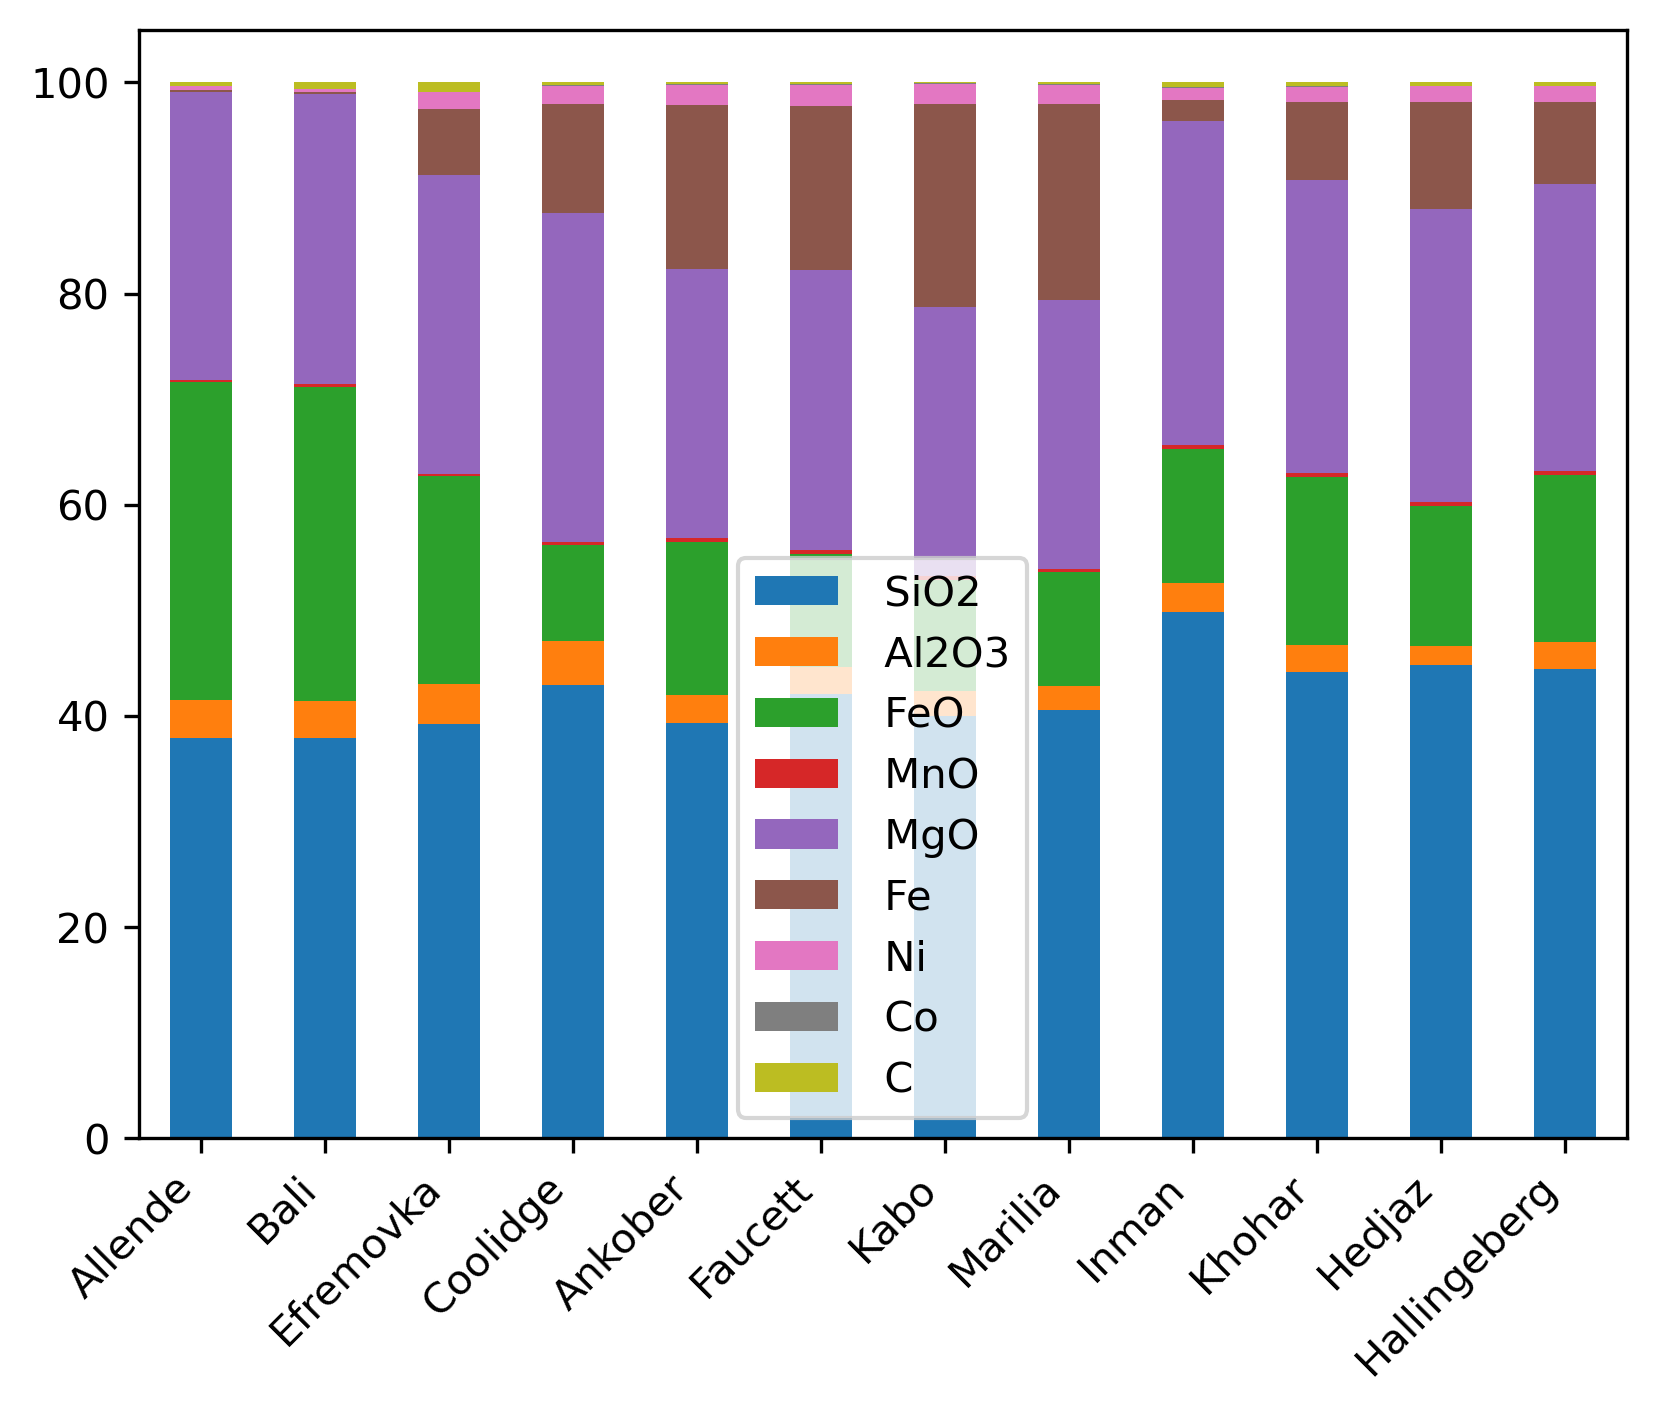
\includegraphics[width=0.8\textwidth]{figures/stacked_bar.png}
    \caption{Example plot showing the chemical composition of meteorites.}
    \label{fig:stacked}
\end{figure}




\section{Exploratory data analysis}\label{sec: Exploratory} % (fold)

To further explore patterns in the data, a Principal Component Analysis (PCA) was performed by singular value decomposition on the meteorite data.
Because PCA is very sensitive to outliers some procedures had to be performed on the data in advance of the svd. First,
the data was centered by pertubing with the geomtric mean. Next, 
the data total variance of the data was calculated and the data was scaled by this metric. Finally, 
the data was CLR-transformed; this step ensures that the Euclidean distance metric implied in the SVD is valid for our data.  

The PCA has been visualised using a biplot and screeplot in Fig. \ref{fig:pcabiplot}. The biplot shows the first two principal components of the data with the samples
represented as points and the variables as arrows. The length of the arrow indicates the importance of the variable in the PCA, and the angle between the arrows indicates how correlated they are.
The screeplot shows the proportion of variance explained by each principal component, which is useful for determining how many components to retain in the analysis. 

The scree plot shows that with only two components, we can explain 96\% of the variance in the dataset, indicating that the decomposition is highly useful for further analysis





\begin{figure}[htbp]
    \centering
    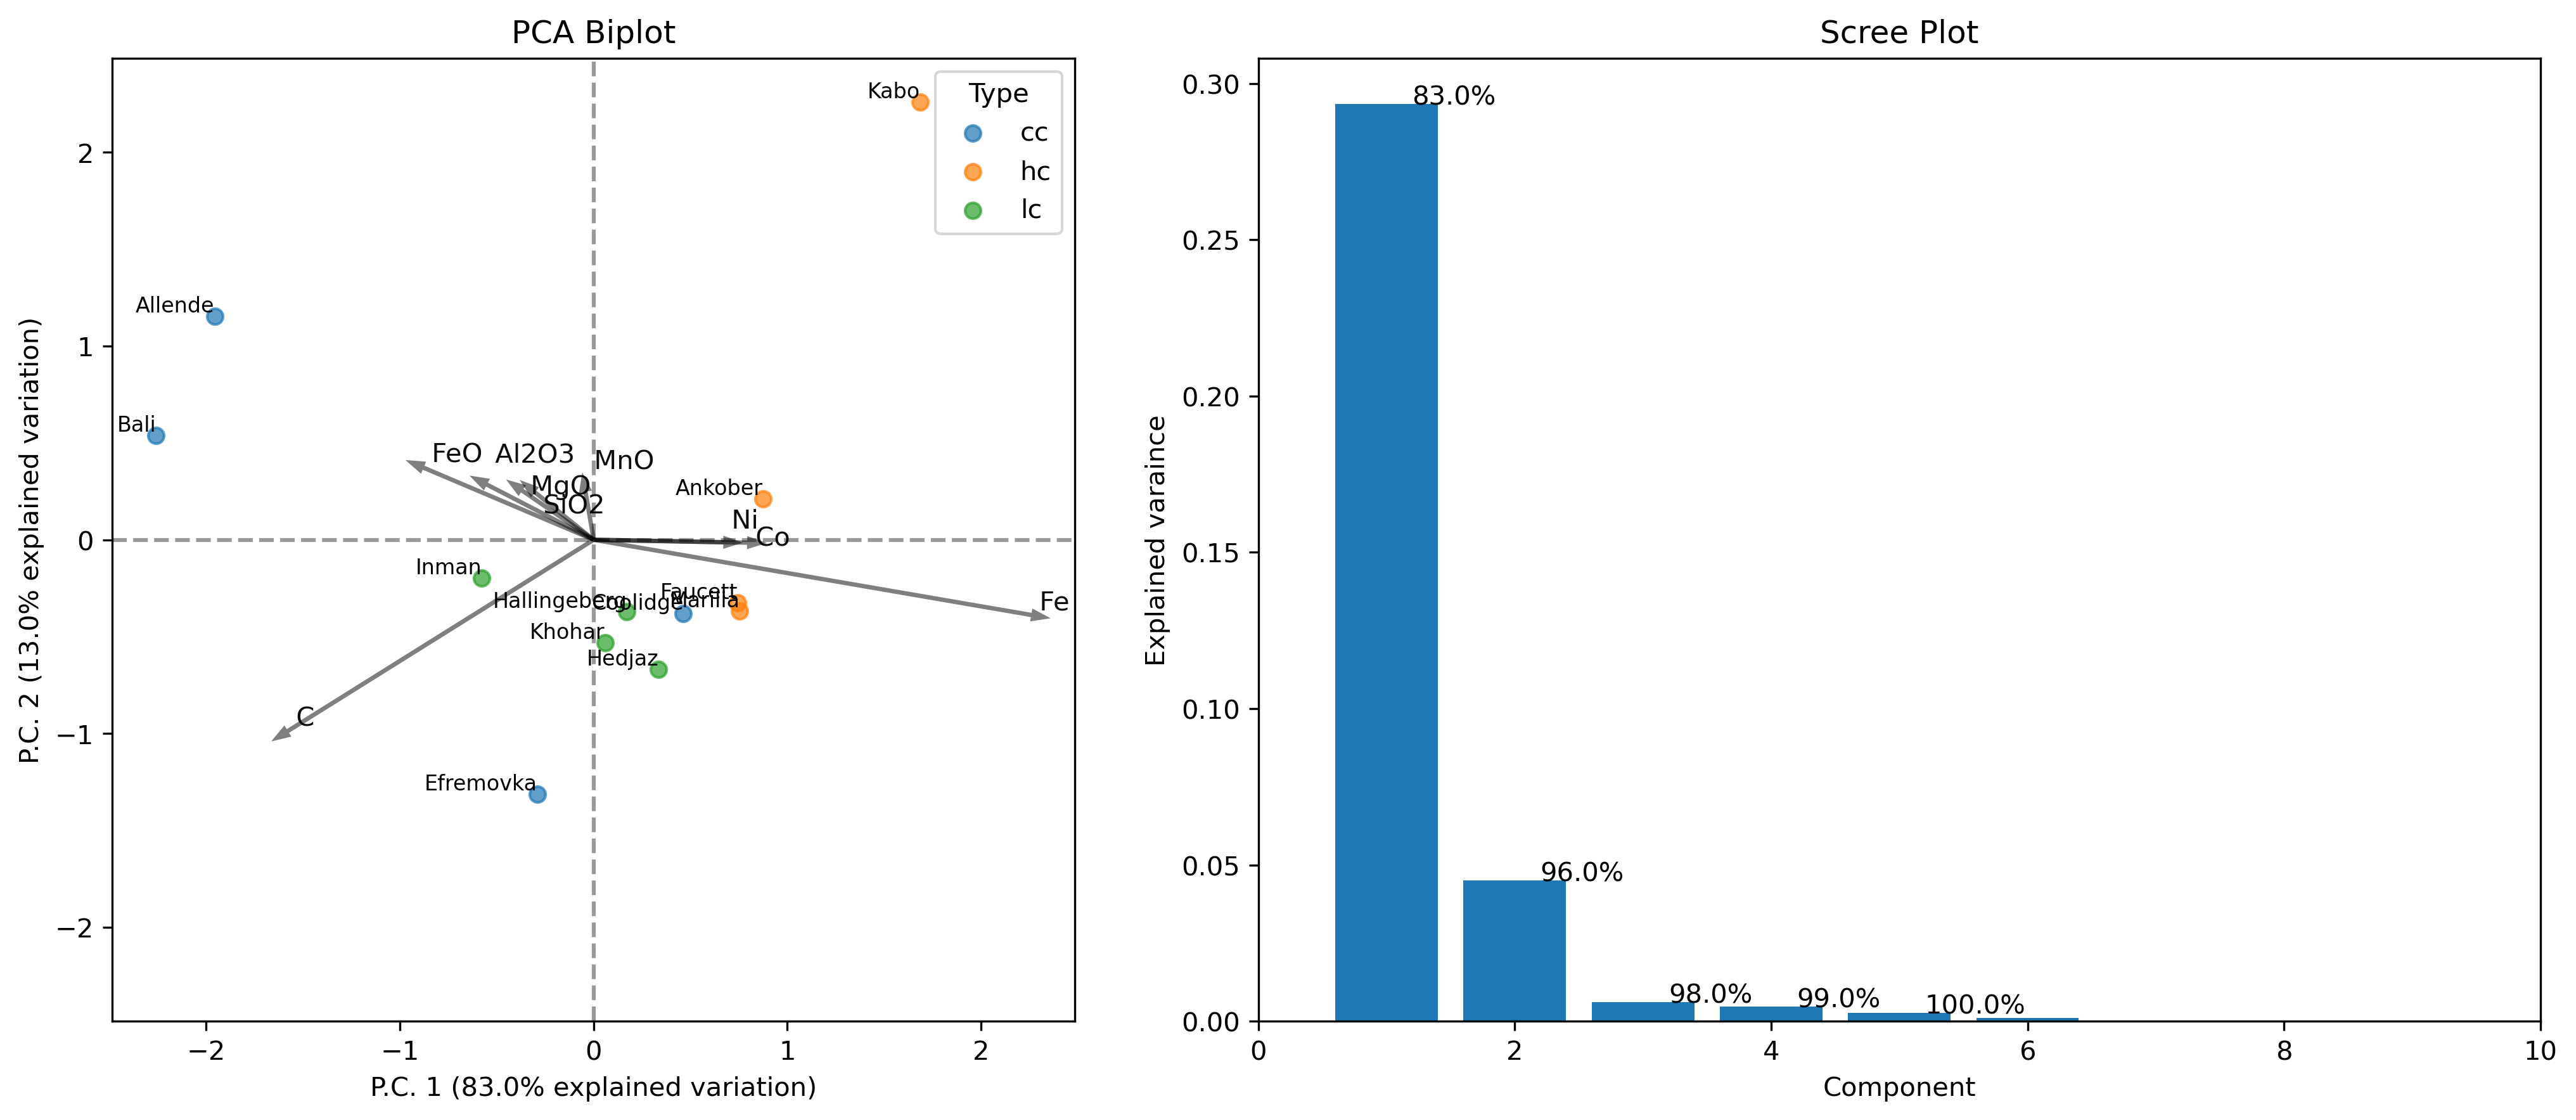
\includegraphics[width=0.8\textwidth]{figures/pca_biplot.png}
    \caption{Example plot showing the chemical composition of meteorites.}
    \label{fig:myplot}
\end{figure}
 %

% section  (end)









%------------------------------------------------------------------------------------%
\newpage{}

\section{Notes}

Deadline: 12/5 kl. 14

5-10 pages incl. Figures

No collaboration


Dataset 2: Simple. No zeros. Look up metadata: cc, hc, lc \newline


 
\subsection{Week5 - Chapter5 - Visualisation} 
\subsection{Week6 - Chapter4 - Zero replacement} 
\subsection{Week7 - Chapter6 - Exploratory data analysis } 
\subsection{Week9 - Chapter8 - Linear analysis ANOVA} 


\section{Title}

\end{document}
